SEE APPENDIX MEI REF LATER
\subsubsection*{In Class Analysis}
\textbf{Question 1}
\begin{figure}[H]
     \centering
     \begin{subfigure}[b]{0.49\textwidth}
         \centering
         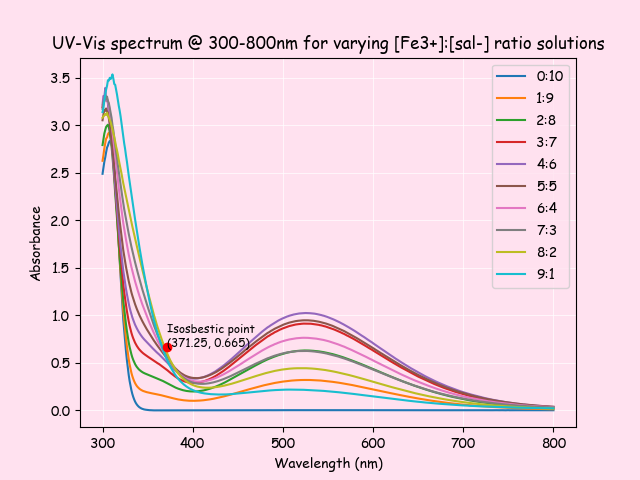
\includegraphics[width=\textwidth]{part2_q1a.png}
         \caption{Varying ratio solutions}
         \label{fig:part2_q1_a}
     \end{subfigure}
     \hfill
     \begin{subfigure}[b]{0.49\textwidth}
         \centering
         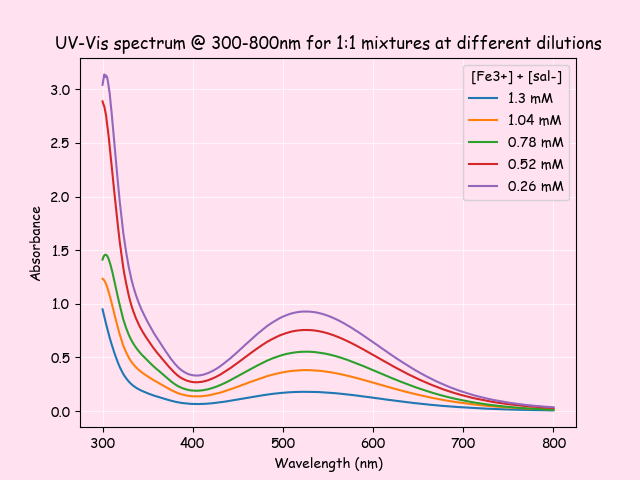
\includegraphics[width=\textwidth]{part2_q1_b.png}
         \caption{Varying concentrations of 1:1 ratio solutions}
         \label{fig:part2_q1_b}
     \end{subfigure}
     \caption{UV-Vis spectrum @ 300 - 800 nm}
     \label{fig:part2q1}
\end{figure}
Isosbestic point was found to be \hl{$\input{part2_q1a.txt}\unskip$}, by averaging the points of intersection for each subsequent solution for those where Fe$^{3+}$ is in excess (6:4 - 10:1). (See Appendix \ref{appx:part2_code} for Python code)
\\
\textbf{Question 2}
\begin{figure}[H]
    \centering
    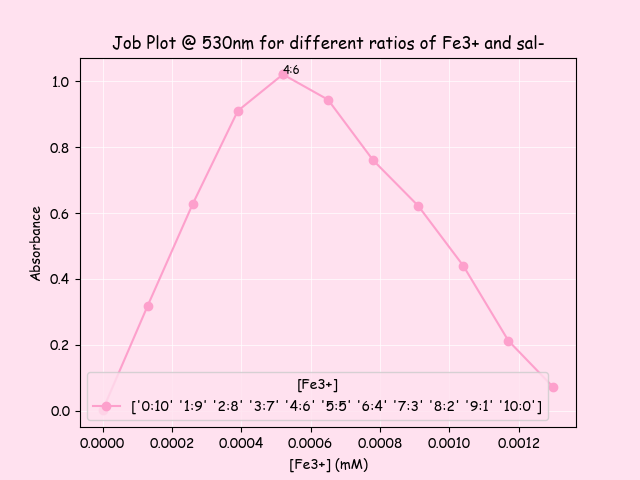
\includegraphics[width = 0.6\linewidth]{part2_q2_job_plot.png}
    \caption{Caption}
    \label{fig:part2q2}
\end{figure}
The ratio at which the peak of Job plot occurred was at a ratio of \input{part2_q2.txt}(2:3). Thus, the empirical formula of the complex was found to be:
\begin{equation}
\mathcolorbox{Lavender}{\ce{[(Fe^{3+})_{2}(sal^-)_3]}}
    \label{eq:emp_formula}
\end{equation}
This does not align with expected values. \hl{ELABORATE}
\\
\textbf{Question 3}
\begin{figure}[H]
    \centering
    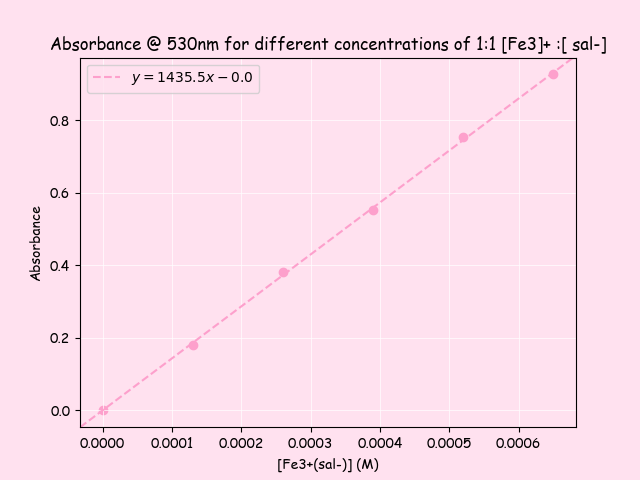
\includegraphics[width = 0.6\linewidth]{part2_q3.png}
    \caption{Caption}
    \label{fig:part2q3}
\end{figure}
From equation (17) of the lab manual\autocite{lab_manual},
\begin{equation}
A = \epsilon_c c_c l
    \label{eq:beer_law}
\end{equation}
Using $l = 1$ cm, the slope of the curve in Figure \ref{fig:part2q3} is the extinction coefficient:
\begin{equation}
   \mathcolorbox{Lavender}{ \epsilon_c = \input{part2_q3.txt} \text{ M}^{-1}\text{cm} ^ {-1}}
    \label{eq:part2_ext_coeff}
\end{equation}
\\
\textbf{Question 4}
CONC OF COMPLEX IS HALF OF THOSE THINGS BC USE SALYCILIC ADN FE
\begin{figure}[H]
     \centering
     \begin{subfigure}[b]{0.49\textwidth}
         \centering
         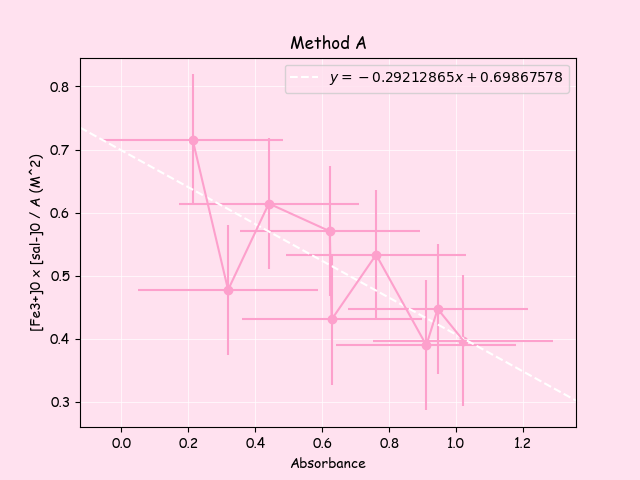
\includegraphics[width=\textwidth]{part2_q4a.png}
         \caption{RENAME}
         \label{fig:part2_q4_a}
     \end{subfigure}
     \hfill
     \begin{subfigure}[b]{0.49\textwidth}
         \centering
         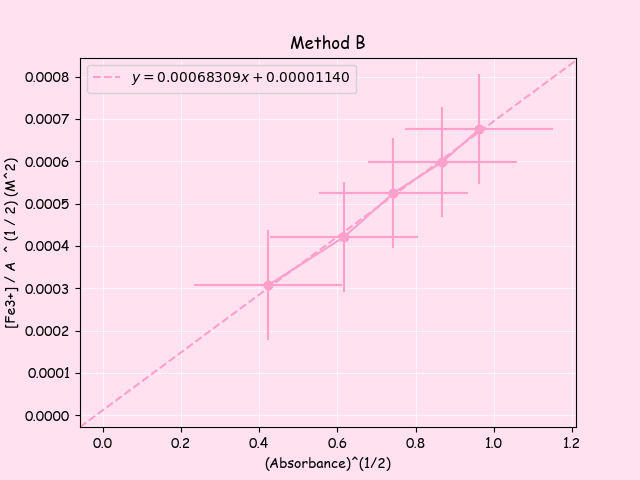
\includegraphics[width=\textwidth]{part2_q4b.png}
         \caption{REDO}
         \label{fig:part2_q4_b}
     \end{subfigure}
     \caption{sjdfsdn}
     \label{fig:part2q4}
\end{figure}

\noindent \textit{Method A}
so much scatter / noise making wonky
\begin{equation*}
    \mathcolorbox{Lavender}{K = \input{part2_q4_a_stab.txt}}
\end{equation*}
\begin{equation*}
    \mathcolorbox{Lavender}{\Delta G^{\circ} = \input{part2_q4_a_gibbs.txt} \text{ Jmol}^{-1}}
\end{equation*}
\begin{equation*}
    \mathcolorbox{Lavender}{\epsilon_c = \input{part2_q4_a_ext.txt}\text{ M}^{-1}\text{cm} ^ {-1}}
\end{equation*}
\textit{Method B}
\begin{equation*}
    \mathcolorbox{Lavender}{K = \input{part2_q4_b_stab.txt}}
\end{equation*}
\begin{equation*}
    \mathcolorbox{Lavender}{\Delta G^{\circ} = \input{part2_q4_b_gibbs.txt} \text{ Jmol}^{-1}}
\end{equation*}
\begin{equation*}
    \mathcolorbox{Lavender}{\epsilon_c = \input{part2_q4_b_ext.txt}\text{ M}^{-1}\text{cm} ^ {-1}}
\end{equation*}